% LTeX: language=it_IT

\documentclass[main.tex]{subfiles}
\graphicspath{{../Figures/Dolci/}}

\begin{document}
    \chapter{Dolci}

    \newpage % Salame di Cioccolato
    \begin{recipe}
        [%
            preparationtime = {\unit[30]{min}},
            portion = {\unit[12]{Porzioni}},
            source = {Nonna Maria Teresa},
        ]
        {Salame di Cioccolato}

        \graph{
            big = placeholder.jpeg
        }

        \ingredients{
            \unit[250]{g} & Biscotti Oro Saiwa \\
            \unit[100]{g} & Burro \\
            2 & Uova \\
            \unit[50]{g} & Cacao amaro \\
            \unit[150]{g} & Zucchero \\
            \unit[1]{bicchierino} & Rhum
        }

        \preparation{
            \begin{enumerate}
            \item Spezzettate i biscotti e bagnateli con il rhum.
            \item In una ciotola lavorate il burro ammorbidito con lo zucchero, aggiungete le uova, il cacao e i biscotti sbriciolati.
            \item Formate un salame con l'impasto, avvolgetelo nella pellicola trasparente e mettetelo in frigorifero per almeno un'ora prima di servirlo.
            \end{enumerate}
        }
    \end{recipe}

    \newpage % Torta di Mele
    \begin{recipe}
        [%
            preparationtime = {\unit[30]{min}},
            bakingtime = {\unit[40]{min}},
            portion = {\unit[12]{Porzioni}},
            source = {Nonna Maria Teresa},
        ]
        {Torta di Mele}

        \graph{
            big = TortaMele.jpeg
        }

        \ingredients{
            \unit[250]{g} & Biscotti Oro Saiwa (circa 32) \\
            \unit[160]{g} & Zucchero \\
            \unit[100]{g} & Farina \\
            \unit[0.8]{bicchiere} & Latte \\
            \unit[1]{bicchierino} & Rhum \\
            \unit[1]{bustina} & Lievito per dolci \\
            1 & Uovo \\
            \unit[250]{g} & Uva passa \\
            \unit[1]{bustina} & Pinoli \\
            3 & Noci \\
            \unit[500]{g} & Mele
        }

        \preparation{
            \begin{enumerate}
            \item Spezzettate i biscotti e metteteli a bagno nel latte e il Rhum. Mescolate fino a ottenere un pastone.
            \item Setacciate la farina con il lievito e aggiungetela al composto di biscotti. Aggiungete lo zucchero, l'uovo, l'uva passa, i pinoli e le noci tritate.
            \item Sbucciate le mele, tagliatele a fettine sottili e incorporatele al composto.
            \item Versate il composto in una tortiera imburrata e infarinata e cuocete in forno preriscaldato a \unit[170]{°C} per circa \unit[40]{minuti}.
            \end{enumerate}
        }
    \end{recipe}

    \newpage % Plumcake
    \begin{recipe}
        [%
            preparationtime = {\unit[30]{min}},
            bakingtime = {\unit[1]{ora}},
            portion = {\unit[12]{Porzioni}},
            source = {Nonna Maria Teresa},
        ]
        {Plumcake}

        \graph{
            big = placeholder.jpeg
        }

        \ingredients{
            \unit[100]{g} & Burro \\
            \unit[150]{g} & Zucchero \\
            \unit[180]{g} & Farina \\
            \unit[100]{g} & Uvetta \\
            2 & Uova \\
            2 & Tuorli \\
            \unit[1]{bicchierino} & Rhum \\
            \unit[1]{bustina} & Lievito per dolci \\
            1 & Limone (scorza grattugiata)
        }

        \preparation{
            \begin{enumerate}
            \item Nota: se non sapete cosa fare con gli albumi avanzati, potete prepararci delle meringhe. Altrimenti usate 3 uova intere.
            \item Ammollate l'uvetta in acqua.
            \item Lavorate il burro ammorbidito con lo zucchero.
            \item Setacciate la farina con il lievito e aggiungetela al composto di burro e zucchero. Aggiungete le uova, i tuorli, la scorza di limone grattugiata e il Rhum. Mescolate bene.
            \item Asciugate l'uvetta e infarinatela leggermente, quindi unitela al composto.
            \item Versate il composto in uno stampo da plumcake imburrato e infarinato e cuocete in forno preriscaldato a \unit[150]{°C} per circa \unit[1]{ora}. Il plumcake è pronto quando, toccando la pasta con un dito, non si sente più sfrigolio.
            \end{enumerate}
        }
    \end{recipe}

    \newpage % Torta Sacher
    \begin{recipe}
        [%
            preparationtime = {\unit[1]{ora}},
            bakingtime = {\unit[45]{min}},
            portion = {\unit[12]{Porzioni}},
            source = {Nonna Maria Teresa},
        ]
        {Torta Sacher}

        \graph{
            big = TortaSacher.jpeg
        }

        \ingredients{
            4 & Uova \\
            \unit[240]{g} & Farina \\
            \unit[250]{g} & Zucchero \\
            \unit[70]{g} & Burro \\
            \unit[60]{g} & Cacao amaro \\
            \unit[250]{ml} & Latte \\
            \unit[1]{bustina} & Lievito per dolci \\
            \unit[100]{g} & Cioccolato fondente \\
            \unit[200]{g} & Marmellata di albicocche \\
            & Panna montata (per servire)
        }

        \preparation{
            \begin{enumerate}
                \item Lavorate il burro ammorbidito con lo zucchero fino a ottenere una crema.
                \item Separate i tuorli dagli albumi. Aggiungete i tuorli all'impasto, continuando a mescolare.
                \item Setacciate la farina con il cacao e il lievito, quindi unite il latte. Amalgamate bene usando una frusta per rompere eventuali grumi.
                \item Unite i due composti, mescolando bene.
                \item Montate gli albumi a neve ben ferma e uniteli delicatamente al composto. Usate movimenti dal basso verso l'alto con una spatola per non smontare gli albumi.
                \item Versate il composto in una tortiera (diametro \unit[24]{cm}) imburrata e infarinata e cuocete in forno preriscaldato a \unit[180]{°C} per circa \unit[45]{minuti}.
                \item Una volta raffreddata, tagliate la torta a metà e farcitela con la marmellata di albicocche.
                \item Sciogliete il cioccolato a bagnomaria e versatelo sulla torta, spalmando con una spatola per ricoprirla completamente.
                \item Lasciate raffreddare per almeno un ora.
                \item Servite la torta Sacher accompagnata da panna montata.
            \end{enumerate}
        }
    \end{recipe}

    \newpage % Crostata
    \begin{recipe}
        [%
            preparationtime = {\unit[45]{min}},
            bakingtime = {\unit[45]{min}},
            portion = {\unit[8]{Porzioni}},
            source = {Claudia},
        ]
        {Crostata}

        \graph{
            big = Crostata.jpeg
        }

        \ingredients{
            \unit[300]{g} & Farina \\
            \unit[135]{g} & Burro \\
            \unit[80]{g} & Zucchero \\
            \unit[1]{bustina} & Lievito per dolci \\
            2 & Uova \\
            1/2 & Limone (scorza grattugiata) \\
            & Marmellata (a piacere)
        }

        \preparation{
            \begin{enumerate}
            \item Lavorate il burro ammorbidito con lo zucchero.
            \item Setacciate la farina con il lievito e unitela al composto, impastando con le mani fino a ottenere un impasto sabbioso.
            \item Aggiungete le uova e la scorza grattugiata di limone e impastate bene.
            \item Fate una palla, avvolgete l'impasto nella pellicola trasparente e lasciatelo riposare in frigorifero per almeno \unit[1]{ora}.
            \item Usate 2/3 dell'impasto per foderare una tortiera imburrata e infarinata (o rivestita con carta da forno).
            \item Farcite con la marmellata a piacere.
            \item Con la pasta avanzata, create delle strisce per decorare la crostata.
            \item Cuocete in forno preriscaldato a \unit[180]{°C} per circa \unit[45]{minuti}.
            \end{enumerate}
        }
    \end{recipe}

    \newpage % Varianti crostata
    \section*{Varianti}
        \subsection*{Crostata speziata}
            % 2 columns with figure on left and text on right
            \begin{multicols}{2}
                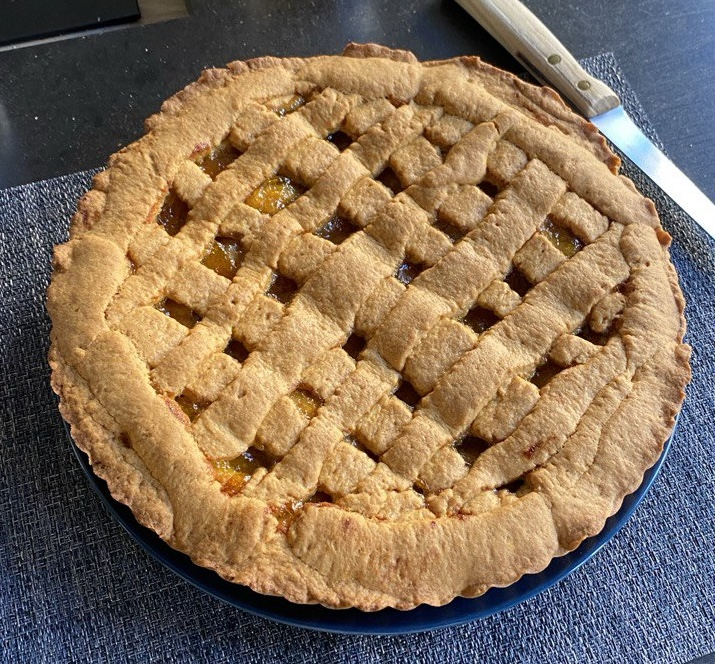
\includegraphics[width=0.4\textwidth]{CrostataSpeziata.jpeg}
                \columnbreak
                \\ Aggiungete all'impasto un cucchiaino di curcuma, un pizzico di pepe e i semi di un cardamomo verde tritati finemente.
            \end{multicols}
        \subsection*{Crostata al cacao}
            \begin{multicols}{2}
                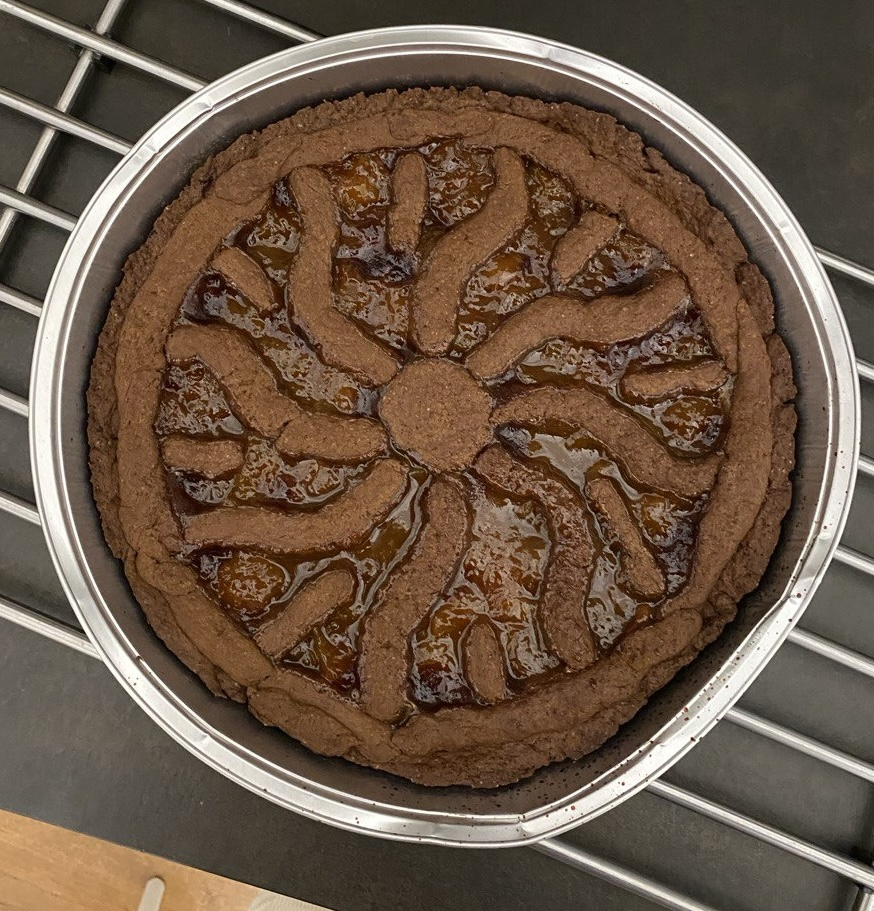
\includegraphics[width=0.4\textwidth]{CrostataCacao.jpeg}
                \columnbreak
                \\ Sostituite \unit[50]{g} di farina con \unit[50]{g} di cacao amaro in polvere.
            \end{multicols}
        \subsection*{Crostata alla Crema}
            \begin{multicols}{2}
                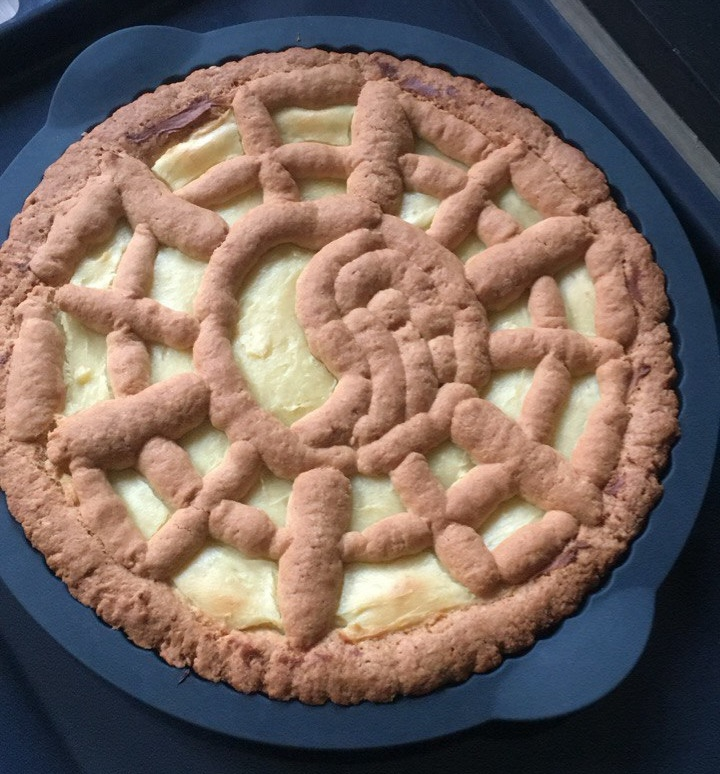
\includegraphics[width=0.4\textwidth]{CrostataCrema.jpeg}
                \columnbreak
                \\ Sostituite la marmellata con della crema pasticcera. In questo caso, Infornate la base di pasta frolla per \unit[15]{minuti} prima di aggiungere la crema, poi cuocete per altri \unit[25]{minuti}.
            \end{multicols}
            

    \newpage % Biscoti Zaeti
    \begin{recipe}
        [%
            preparationtime = {\unit[30]{min}},
            bakingtime = {\unit[20]{min}},
            portion = {\unit[6]{Porzioni}},
            source = {Barcelona, 20/01/2026},
        ]
        {Biscotti Zaeti}

        \graph{
            big = Zaeti.jpeg
        }

        \ingredients{
            \unit[140]{g} & Farina di mais gialla \\
            \unit[100]{g} & Farina 00 \\
            \unit[75]{g} & Zucchero \\
            \unit[70]{g} & Burro \\
            1 & Uova \\
            \unit[50]{g} & Uvetta \\
            \unit[1/2]{bustina} & Lievito per dolci \\
            \unit[1]{bicchierino} & Vino bianco dolce \\
            \unit[1]{cucchiaino} & curcuma \\
            \unit[1]{pizzico} & Pepe nero
        }

        \preparation{
            \begin{enumerate}
            \item Ammollate l'uvetta nel vino bianco.
            \item Lavorate con le mani il burro ammorbidito con lo zucchero, le farine e il lievito. Fino a ottenere un impasto sabbioso.
            \item Aggiungete l'uovo, la curcuma, il pepe nero e le uvette con il vino, mescolando con una forchetta.
            \item Accendete il forno a \unit[180]{°C}. Preparate una teglia rivestita con carta da forno.
            \item Formate delle palline con l'impasto e schiacciatele leggermente, formando dei dischetti. Disponendoli sulla teglia.
            \item Cuocete per circa \unit[20]{minuti}. Quando sfornate, i biscotti devono essere leggermente morbidi.
            \item Lasciate raffreddare i biscotti su una gratella prima di servirli.
            \end{enumerate}
        }
    \end{recipe}

\end{document}